\chapter{Results}
\label{chapter:results}
In this chapter, we apply the advanced statistical tools to the heavy-flavor transport model and extract the heavy quark transport coefficients.
I would like to present this in a two step processes to show the improvements of the lastest extraction.



\paragraph{A list of experimental data}
\section{Lessons from earlier extractions of $\hat{q}_Q$}
In an earlier publication [], we used a linearized Boltzmann model with the coherence factor approach to implement the LPM effect.
The heavy quark initial momentum dsitribution is obtained from the FONLL calculation.
We have already commented on the advantages and disadvantages of these choices.
Two different set of nuclear PDF $EPPS$ and $nCTEQ15$ are used to represent the uncertainty from the cold nuclear matter effect in the $\hat{q}$ extraction.

Regarding model parameters, the one parameter for the perturbative elastic and inelastic scatterings is controlled by $1/3 < \mu < 4$ in the running coupling. 
There is an additional pure diffusion process with a diffusion constant $\kappa_{NP}$ parametized to peak at low temperature and low energy, in order to mimic certain non-perturbative coupling between a low energy probe and the medium near $T_c$,
\begin{eqnarray}
\kappa_{NP} = T^3 \kappa_D \left(x_D + (1-x_D)\frac{1\textrm{ GeV}{}^2}{ET}\right).
\end{eqnarray}
The $0<\kappa_D<8$ parameter is the overall strength of the diffusion, and the $0<x_D<1$ controls the degree of energy-temperature dependence.
One can see that in the heavy quark limit $M\rightarrow \infty$, this parametrization becomes independent of mass.
An additional parameter is the in-medium energy loss starting time $\tau_0$ that is allowed to be tuned between $0.1$ fm/$c$ to $1.0$ fm/$c$ (before the onset of hydrodynamics).
The reason is we lack a quantitative description of the production of color charge in the initial stages.
This starting time is a simple approximation that interactions is only turned on after $\tau_0$ when the color carries is assumed to approach a Boltzmann distribution.


The design of the four dimensional parameter space  $(\tau_0, \mu, \kappa_D, x_D)$ has 80 design points.
The computation is carried on the distributed computing system Open Science Grid [] using about a million CPU hours.
The observabes on which we calibrated are listed in tables \ref{table:ALICE-obs} and \ref{table:CMS-obs}. 
Including, $p_T$ dependent $D$-meson nuclear modification factor $R_{AA}$ and $p_T$ dependent (event-shape-engineered) azimuthal anisotropy $v_2$.
CMS measurements of the $B^{\pm}$-meson $R_{AA}$ is also included to constrain the mass dependence of the transport coefficients.

\begin{figure*}
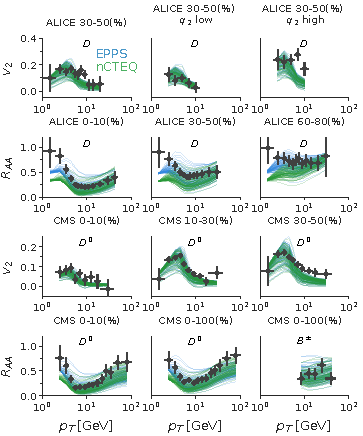
\includegraphics[width=.49\textwidth]{observables_design.pdf}
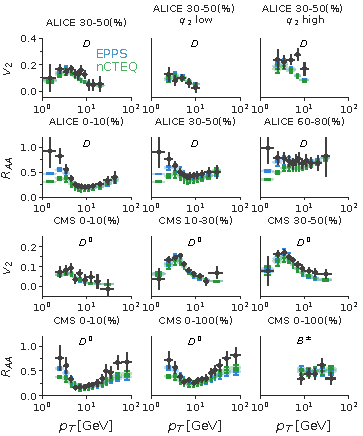
\includegraphics[width=.49\textwidth]{observables_posterior.pdf}
\caption{Left: the prior, i.e. the full range of calculations in parameter space. Right: the posterior, i.e. observables sampled from model emulators after calibration. In both figures, blue (green) lines are calculations with {\tt EPPS} ({\tt nCTEQ15np}) nuclear PDF.}\label{plots:deisgn_posterior_obs}
\end{figure*}

The prior and the posterior of the observables before and after the calibration is shwon in figure \ref{plots:deisgn_posterior_obs}.
blue stands for using {\tt EPPS} nuclear PDF and green stands for using the {\tt nCTEQnp}  nuclear PDF.
We found that the model after the calibration provide a good description of $R_{AA}$ and $v_2$ at the intermediate $p_T$ of the ALICE experiments.
But it does not reproduce the fast uprising shape of $R_{AA}$ at high-$p_T$ of the CMS experiment.
In addition, the model seem to under estimate the high-$p_T$ $v_2$ of the $30-50\%$ centrality bin measured by CMS.
The model is able to explain the correlation between the D-meson $v_2$ and the event-shape, though there are still large fluctuation in the data.
The use of different nuclear PDFs has a negligible effect on $v_2$, but does affect the $R_{AA}$ at small and large $p_T$.
Another thing worth noting that is that the $D$ and $B$ meson $R_{AA}$ are described at the same time.

\begin{figure}
\centering
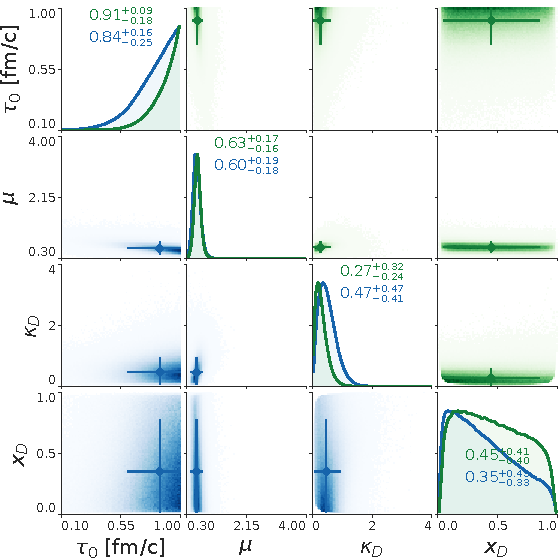
\includegraphics[width=.7\textwidth]{posterior.pdf}
\caption{Marginalized postrior probability distribution of model parameters. Diagonal plots show the marginalization on a single parameter. Off diagonal plots show the pair correlation between parameters. Blue (Geen) lines and lower (upper) off diagonal plots correspond to the extraction using EPPS (nCTEQ15np) nuclear PDF.}\label{plots:posterior}
\end{figure}

The inferred posterior probability distribution of the parameters is shown in the figure \ref{plots:posterior}.
The diagonal plots show single parameterized distributions, and the off-diagonal ones displays the two-parameter correlations.
We split the results that use different nuclear PDFs into the upper (EPPS, green heat map and lines) and lower (nCTEQ15np, blue heat maps and lines) triangles.
One notices that results from different nuclear PDF are consistent within the uncertainty; therefore, from now on I shall not stress on any differences between these two set of results, but combine them into a single distribution to fold in the PDF uncertainty.
The favored parameters are $\mu \sim 0.6$ and $\kappa_D \sim 0.4$, indicating a large in-medium $\alpha_s$ and a small additional diffusion.
The typical value of the $\alpha_s$ is, in fact, so large that let one worried about the use of weakly-couple based approaches.
For example, $\alpha_s(0.6\pi T)$ at $T=300$ MeV is 0.67, corresponding to $g \approx 3$. 
And the screening mass $m_D \sim 3.6 T$ is even larger than the average energy of the thermal partons $3T$. 
In the discussion of the next section, we will see that this problem can be slightly alleviated, once we use the improved implementation of the LPM effect and implement a separation of soft-modes into the diffusion constant, though $g$ is still large.

\begin{figure}
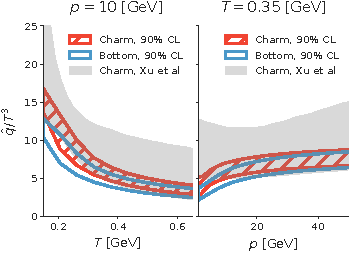
\includegraphics[width=\columnwidth]{qhat_p_T.pdf}
\caption{Posterior range of the heavy quark transverse momentum broadening parameter $\hat{q}$ from Equation \ref{eq:qhat}. The results include the uncertainty from using different nuclear PDFs. Blue boxed region is for bottom quarks and red slashed region for charm quarks.}\label{fig:posterior_qhat}
\end{figure}

\paragraph{Transport coefficients} In this analysis, the heavy quark transport coefficient $\hat{q}$ is computed from adding up the momentum broadening from both the scattering and the parametric diffusion,
\begin{eqnarray}\label{eq:qhat}
\hat{q} &=& 2T^3\kappa_D\left(x_D + (1-x_D)\frac{\textrm{GeV}^2}{ET}\right) + \hat{q}_{\textrm{el}}.
\end{eqnarray}
In a perturbative definition of the transport coefficients, the inelastic process does not contribute to heavy quark transport coefficient at leading order. 
In figure \ref{plots:posterior_qhat}, the 90\% credible region of $\hat{q}$ is shown as a function of temperature at a fixed energy (left), and as function of energy at a fixed temperature (right).
Results for charm (red) and bottom (blue) quarks are labeled by different colors.
The mass difference only causes a small difference in $\hat{q}$.

\begin{figure}
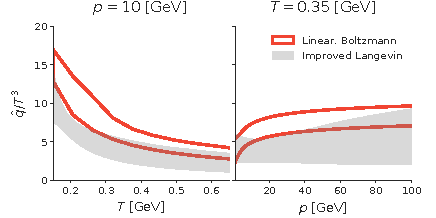
\includegraphics[width=\columnwidth]{qhat_compare.pdf}
\caption{Posterior range of the heavy quark transverse momentum broadening parameter $\hat{q}$. The shaded region indicates a previous extraction using the improved-Langevin model [].}\label{fig:compare_qhat}
\end{figure}

\paragraph{Comparison to results from an improved-Langevin model}
The same transport coefficient is also extracted using the improved-Langevin model [].
It includes a diffusion modeling of the elastic interacton, a high-twist single gluon emission rate, and a similar routine to implement multiple radiations.
This model is then coupled to the same medium as the one used here and compared to the same set of observables as this work does.
The resultant posterior (for charm quark only) is shown as the shaded region in figure \ref{fig:compare_qhat}.
We see that the $\hat{q}$ extracted using the two models only overlap at the boundary of the credible region.
Their difference is comparable to the uncertainty band of either model, while both models provide a reasonable description of the data.
This suggests the theoretical uncertainty that comes from the assumption between the probe and the medium is a significant one.
The ability to tune a switching scale parameter in the new model intends to include this type of theoretical uncertainty.

\section{Calibration using the improved transport model}
Finally, we apply the improved model to the extraction of the heavy quark transport coefficients.
As a summary of the improvements:
\begin{itemize}
\item A more sophisticated implementation of the LPM effect to reduce modeling uncertainty of the radiative process;
\item An interpolation of the diffusion picture and the scattering picture to take into account modeling uncertainty.
\item Separating the high-virtuality evolution and the low-virtuality transport equation at a medium scale.
\end{itemize}

\paragraph{Model parameters}
In the new analysis, we try to include as many theoretical uncertainty as possible, so we have much more parameters than the two previous studies.
They are listed in table \ref{table:new:prior}.
\begin{itemize}
\item The first parameter is again the energy loss starting time $\tau_i$.
In this analysis, we are comparing to data at two collision energies and the hydrodynamic starting time $\tau_0$ varies from $1.2$ fm/$c$ to $0.6$ fm/$c$.
To account for this differences, we use the ratio $\xi = \tau_i/\tau_0$ as the single parameter for both energies.
It means that after $\xi$ fraction of the hydrodynamization time, the color density is assumed to be large enough to apply the linearized transport  model.
\item The second parameter is switching scale parameter $1.0 < c < 10.0$ in $Q_{\textrm{cut}}^2 = c m_D^2$. For a typical coupling $g\sim 2$, $Q_{\textrm{cut}}$ is then varied from about $2T$ to $7T$.
\item The third parameter $0<R_v<7$ controls the matching condition between the vacuum-like radiation and the medium-induce radiation $\Delta k_\perp^2 = R_v Q^2$.
At $R_v = 0$, the vacuum-like radiation is completely forbidden once it interacts with the medium; for $R_v \gg 1$, the vacuum-like radiation is effectively unmodified.
\item The $0.6 < \mu < 10$ parameter controls the in-medium strong coupling $\alpha_s(\max\{Q, \mu\pi T\})$.
\item The rest of the six numbers $K,a,b,p,q, \gamma$ parametrizes a correction to the weakly coupled transport coefficient $\hat{q} + \Delta\hat{q}$, $\hat{q}_L + \Delta\hat{q}_L$,
\begin{eqnarray}
\Delta\hat{q} &=& \frac{K T^3}{\left[1+\left(a\frac{T}{T_c}\right)^p\right]\left[1+\left(b\frac{E}{T}\right)^q\right]}, \\
\Delta\hat{q}_L &=& \left(\frac{E}{M}\right)^\gamma \frac{\Delta\hat{q}}{2}
\end{eqnarray}
$0 < K < 15$ is the overall magnitude of the correction. 
The deviation from the $T^3$ dependence and the energy dependence are parametrized using two dimensionless combinations $T/T_c$, and $E/T$.
The $\gamma$ parameter varied from $-1$ to $1$ allows the correction to be anisotropic.
Note that such a construction goes back to an isotropic diffusion when velocity approaches zero ($E\rightarrow M$).
\end{itemize}
\begin{table}
\centering
\caption{Prior range of parameters}\label{table:new:prior}
\begin{tabular}{ccc}
\hline
Symbol & Description & Range \\
\hline
$\xi = \frac{\tau_0}{\tau_{\textrm{hydro}}}$ & Energy loss starting time & (.1, .9) \\
$c = \frac{Q_{\textrm{cut}}^2}{m_D^2}$ & Soft / hard switching scale & $(.1, 10.)$ \\
$R_v$ & Vacuum / Medium mathcing scale & $(0,7)$\\
$\mu$ & Running $\alpha_s$ stops at $Q = \mu\pi T$ & $(.6, 10)$ \\
$K$ & Magnitude of $\Delta \hat{q}/T^3$ & $(0, 15)$\\ 
$p$ & \multirow{2}{*}{$E$-dependence of $\Delta \hat{q}/T^3$} & $(-2, 2)$\\ 
$a$ &  & $(-1, 1)$\\ 
$q$ & \multirow{2}{*}{$T$-dependence of $\Delta \hat{q}/T^3$}  & $(-.5, 3)$\\ 
$b$ &   & $(-.5, 3)$\\ 
$\gamma$ & $\Delta \hat{q}_L = (E/M)^\gamma\Delta \hat{q}_L$  & (-1, 1)\\ 
\hline
\end{tabular}
\end{table}

\paragraph{Design and prior} 
We chosoe to give $\ln c, \ln R_v, \ln \mu, \ln a$ and $\ln b$ an uniform design and a uniform prior.
Therefore, the original parameter will have a non-uniform design and prior distribution.
The reason is that these parameters either causes a logarithmic slow change in the model and its prior uncertainty is large that it is allowed vary by orders of magnitude.
For example, the $\mu$ parameter enters the logarithmic running of $\alpha_s$ and we can rewrite the maximum possible $\alpha_s$ as,
\begin{eqnarray}
\alpha_{s,\max}(T) = \frac{2\pi}{9}\frac{1}{\ln(\mu) + \ln(\pi T/\Lambda_{\textrm{QCD}})}
\end{eqnarray}
Therefore, we assign a uniform prior to $\ln(\mu)$ so that $\alpha_s$ also varies notable within the prior range.
For the $c$ and $R_v$ parameter, we have seen in the previous benchmark calculation that the $R_{AA}$ and $v_2$ predictions depends fairly weak on the choice of these parameter, therefore they are also given a logarithm prior.
For the $a$ and $b$ parameters, one notice that asymptotically largeness or smallness of these numbers do not change the value of $\Delta \hat{q}$ notably.
By applying the logarithmic prior and design, we can explore both the large and small limits of these numbers while still have enough design points to control the interpolation uncertainty in the physical interesting regions ($a$ and $b$ are of order one). 

\begin{figure}
\centering
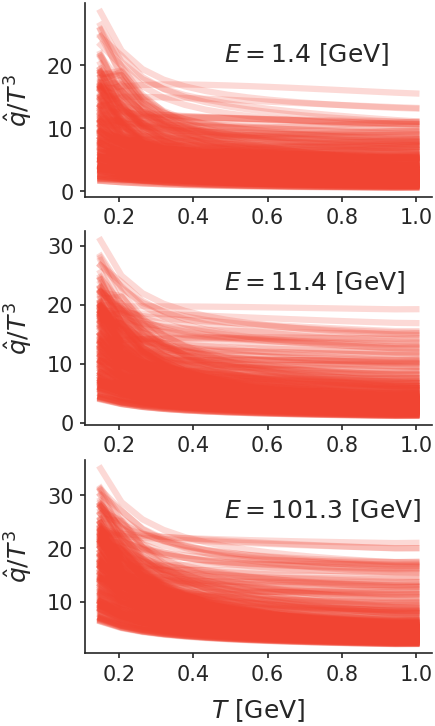
\includegraphics[width=.4\textwidth]{qhat_prior.png}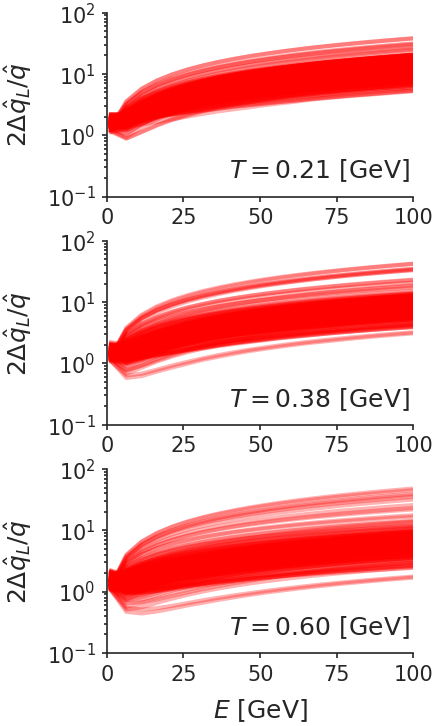
\includegraphics[width=.4\textwidth]{ER_prior.png}
\caption{•}
\label{fig:new:design-qhat}
\end{figure}

We sampled 250 design points and 50 validation points. 
Combining $\mu, K, p, q, a, b$ and $\gamma$, the prior region of the heavy quark transport parameters are plotted function of temperature and energy in figure \ref{fig:new:design-qhat}. 
On the left, 250 design's $\hat{q}$ as function of temperatures are shown  (using charm mass for demonstration).
Each subplot shows quark energy at $1.4$ GeV, $11.4$ GeV and $101.3$ GeV.
The prior range of $\hat{q}$ varies over an order of magnitude.
On the right of the figure, we show the ratio $2\hat{q}_L/\hat{q}$ to indicated the degree of anisotropy of the transport parameters.

The computations of the model on both the design points and the validation points are performed on the NERSC super-computing system using over two million CPU hours.
The prior observables are shown in figure \ref{fig:new:obs_prior_LHC} at LHC energy $\sqrt{s}$ = 5.02 TeV and in figure \ref{fig:new:obs_prior_RHIC} at RHIC energy $\sqrt{s} = 200$ GeV.
In additional to LHC dataset used in the last calibration, we also include a dataset at RHIC energy measured by the STAR Collaboration [].
We choose two observables at RHIC, namely D meson $R_{CP}$ and $v_2$. 
The new one, $R_{CP}$, is defined as the $N_{\textrm{bin}}$ normalized ratio between the D meson yield in a smaller centrality class $C$ to a larger centrality class $P$,
\begin{eqnarray}
R_{\textrm{CP}} = \frac{dN_\textrm{C}/dp_T N_{\textrm{bin,P}}}{dN_\textrm{P}/dp_T N_{\textrm{bin,C}}}.
\end{eqnarray}
Using the nuclear data as a reference has the advantage of canceling certain theoretical uncertainties, such as the nuclear PDF (if its impact-parameter dependence is neglected) and possible modifications to the initial production mechanism in the nuclear environment.
A problem we found at RHIC energy is that even varying wildly the parameters, the very low-$p_T$ $R_{CP}$ is not well covered by the calculation. 
This indicates the model will have to be improved in this region of $p_T$, possible a more up-to-date dynamical hadronization model.
Our temporary solution is to only include the STAR $R_{CP}$ data above $5$ GeV in the calibration.

\begin{figure}
\centering
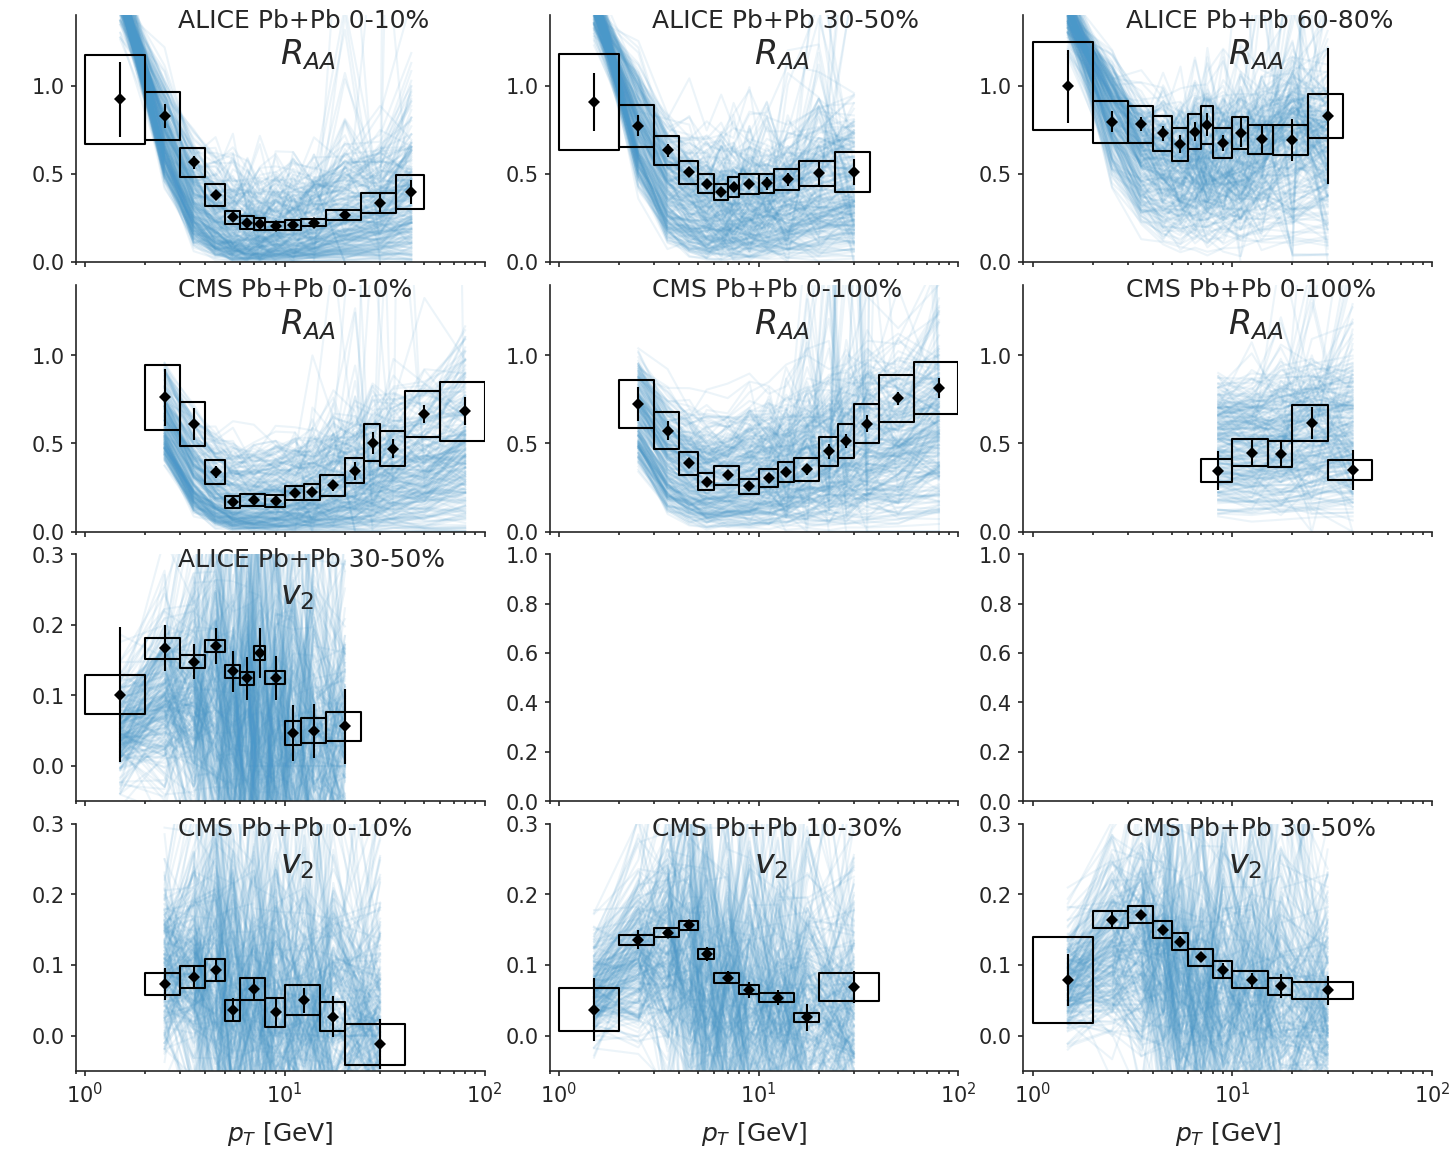
\includegraphics[width=\textwidth]{obs_prior_LHC.png}
\caption{•}
\label{fig:new:obs_prior_LHC}
\end{figure}

\begin{figure}
\centering
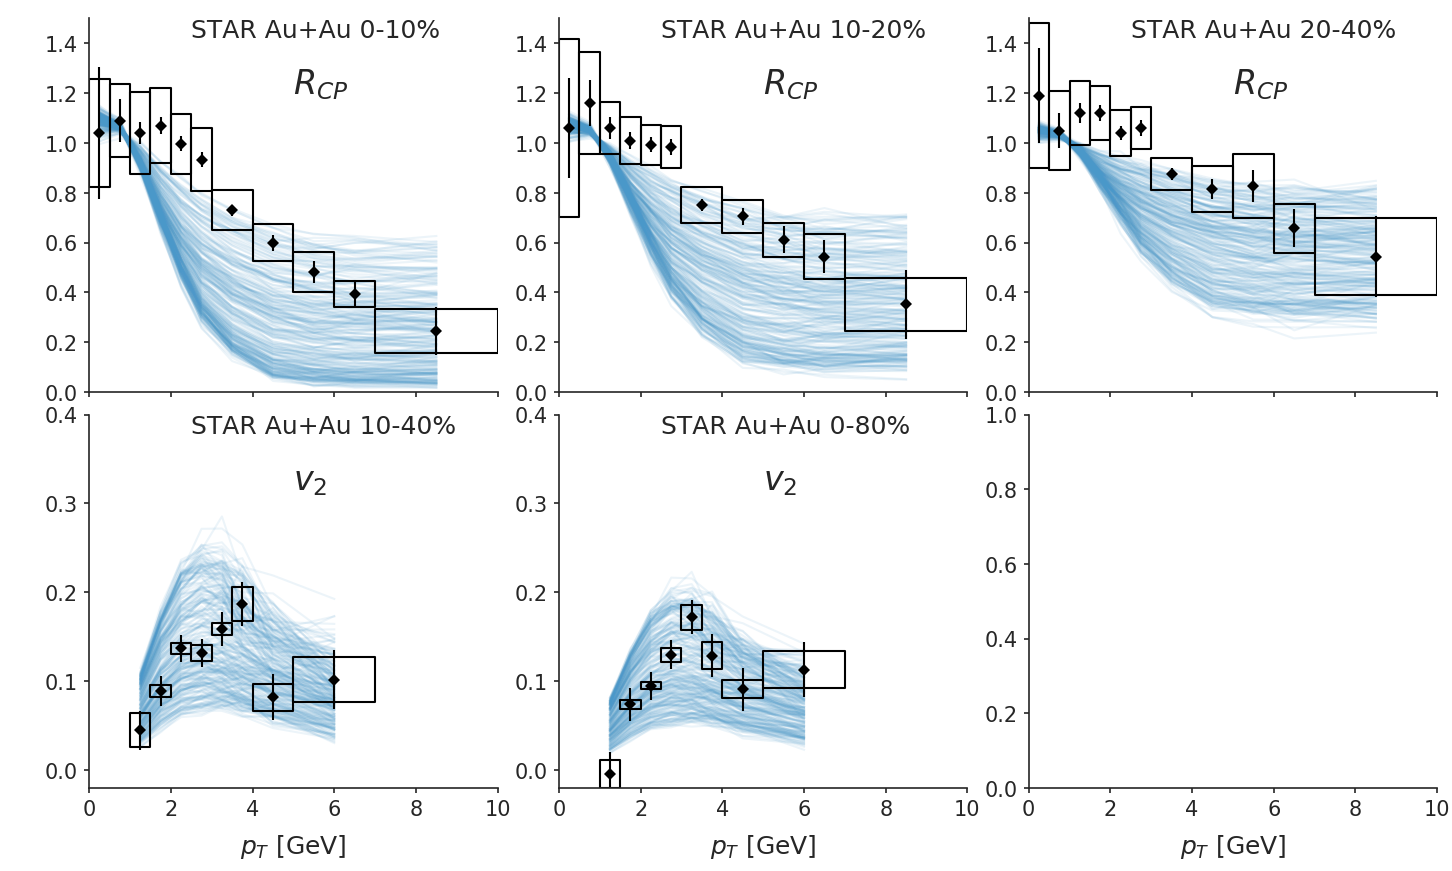
\includegraphics[width=\textwidth]{obs_prior_RHIC.png}
\caption{•}
\label{fig:new:obs_prior_RHIC}
\end{figure}

\paragraph{Emulator validation} 
The validation is performed by comparing the emulator trained on the 250 design points to the actual calculation on the 50 validation points.
We visualize the validation in figure \ref{fig:new:validation}.
In the top row, the emulated $v_2$ (left) and emulated $R_{AA}$ (right) are compared with the model calculations, and the data from different experiments and centrality has been labeled by different colors.
The emulated values strongly correlates with the true calculations around the the $y=x$ line.
Most points hit off the line, meaning the emulator is not 100\% accurate.
To see if the uncertainty is accounted for, we scatter plot the emulator's prediction uncertainty ($1\sigma$, $y$ axis) versus the absolute deviation between the prediction and the calculation (the $x$ axis).
The dashed line defines the shaded region where the true deviation is large than $\pm 3\sigma$.
We found that over $99\%$ of the prediction are within the $3\sigma$ region.
Therefore, for most cases the emulator correctly estimates its uncertainty  and therefore prevents over-fitting.

\begin{figure}
\centering
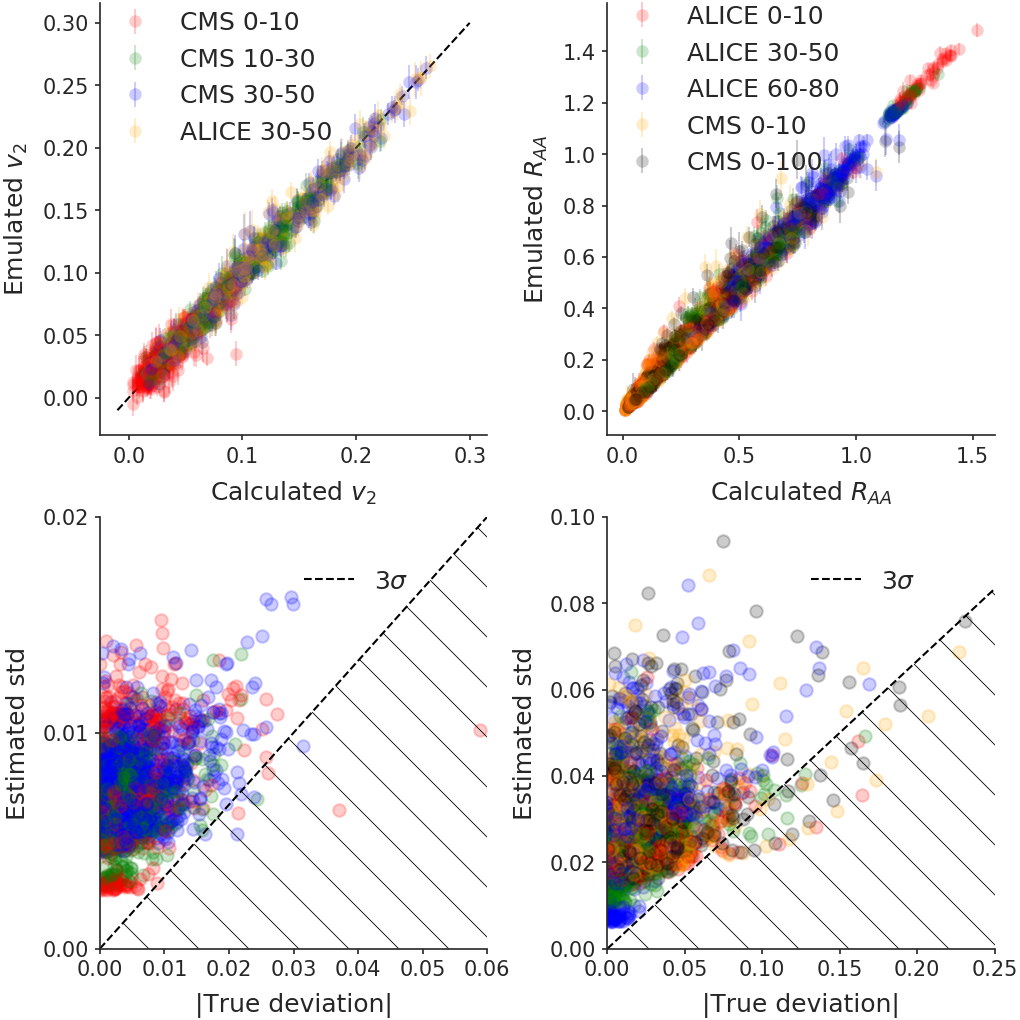
\includegraphics[width=.8\textwidth]{validation.png}
\caption{•}
\label{fig:new:validation}
\end{figure}

\paragraph{Co-variance matrix} 
From chapter \ref{chapter:bayes}, the co-variance matrix has the structure
\begin{eqnarray}
\Sigma = \Sigma_{\textrm{emulator}} + \Sigma_{\textrm{truncation}} + \Sigma_{\textrm{stat}} + \Sigma_{\textrm{sys}} + \Sigma_{\textrm{model, sys}} 
\end{eqnarray}
The construction of these terms are straight forward, except for the systematic covariance $\Sigma_{\textrm{sys}}$ of the experimental data.
Usually, experiments publish the marginalized uncertainty on each observable point $\delta y_{sys}$ (for example, $R_{AA}$ of a certain centrality at a single $p_T$ bin), and may specify the nature of the uncertainty as ``correlated'' or ``uncorrelated''.
The correlation among uncertainties is important as it directly affects the interpretation of the quality of fit.
For instance: a fit with $+5\%$ deviations on each of the $N$ data points will be penalized by a factor $e^{-N(0.05 y)^2/\delta y^2}$, assuming uncorrelated uncertainty; while it will only be penalized by $e^{-(0.05 y)^2/\delta y^2}$ if one assumes fully correlated uncertainty.
This is because fully correlated uncertainty allows data to be systematically deviation from a trend.

However, we the lack the information to construct the full covariance matrix from $\delta y_{sys}$.
In this study, we simply parametrize the correlation as function of observables (labeled by $\alpha, \beta \in \{R_{AA}, v_2, R_{CP}\}$), centrality labeled by $m,n$ and transverse momentum (labeled by $i,j$),
\begin{eqnarray}
\mathbf{\Sigma}_{\textrm{sys}} = \delta_{\alpha\beta} C_{mn}  \exp\left\{-\frac{1}{2 L_{\textrm{corr}}^2} \left(\ln\frac{p_{T, i}}{p_{T, j}}\right)^2 \right\} \times \sigma^{\alpha m}_{\textrm{sys}, i}\sigma^{\beta n}_{\textrm{sys}, j}.
\end{eqnarray}
So, the covariance is zero if there are different observables or measurements from different experiments or different particle species.
The centrality correlation $C_{mn}$ is only applied to $R_{AA}$ and $R_{CP}$ as these quantities across different centrality shares the same baseline reference, so a fraction of their uncertainty must be correlated across-centrality. 
By default, $C_{m=n}=1$ and $C_{m\neq n}=0.3$.
The correlation in the $p_T$ dimension is assumed to be a Gaussian in the $\ln p_T$ space with correlation length $L_{\textrm{corr}}$.
We use $\ln p_T$ based on the consideration that the original of these uncertainty should not be sensitive to the linear change of $p_T$ as the there is no other scale present.
The default correlation length is $1$, meaning the uncertainty is effectively uncorrelated with measurements at a $p_T$ $2.7$ times larger or smaller.
Finally, this correlation modulation is applied to the completely correlation case of the systematic uncertainty $\sigma^{\alpha m}_{\textrm{sys}, i}\sigma^{\beta n}_{\textrm{sys}, j}$.

This construction is entirely parametric, except for the direct experimental inputs $\sigma^{\alpha m}_{\textrm{sys}, i}$.
We hope that future measurements will provide more information on the co-variance structure of the published systematic uncertainties.
In the actually calibration, we will also change a few default parameters to see if the extracted physical parameters are sensitive to the detailed construction of $\Sigma_{\textrm{sys}}$.

\begin{figure}
\centering
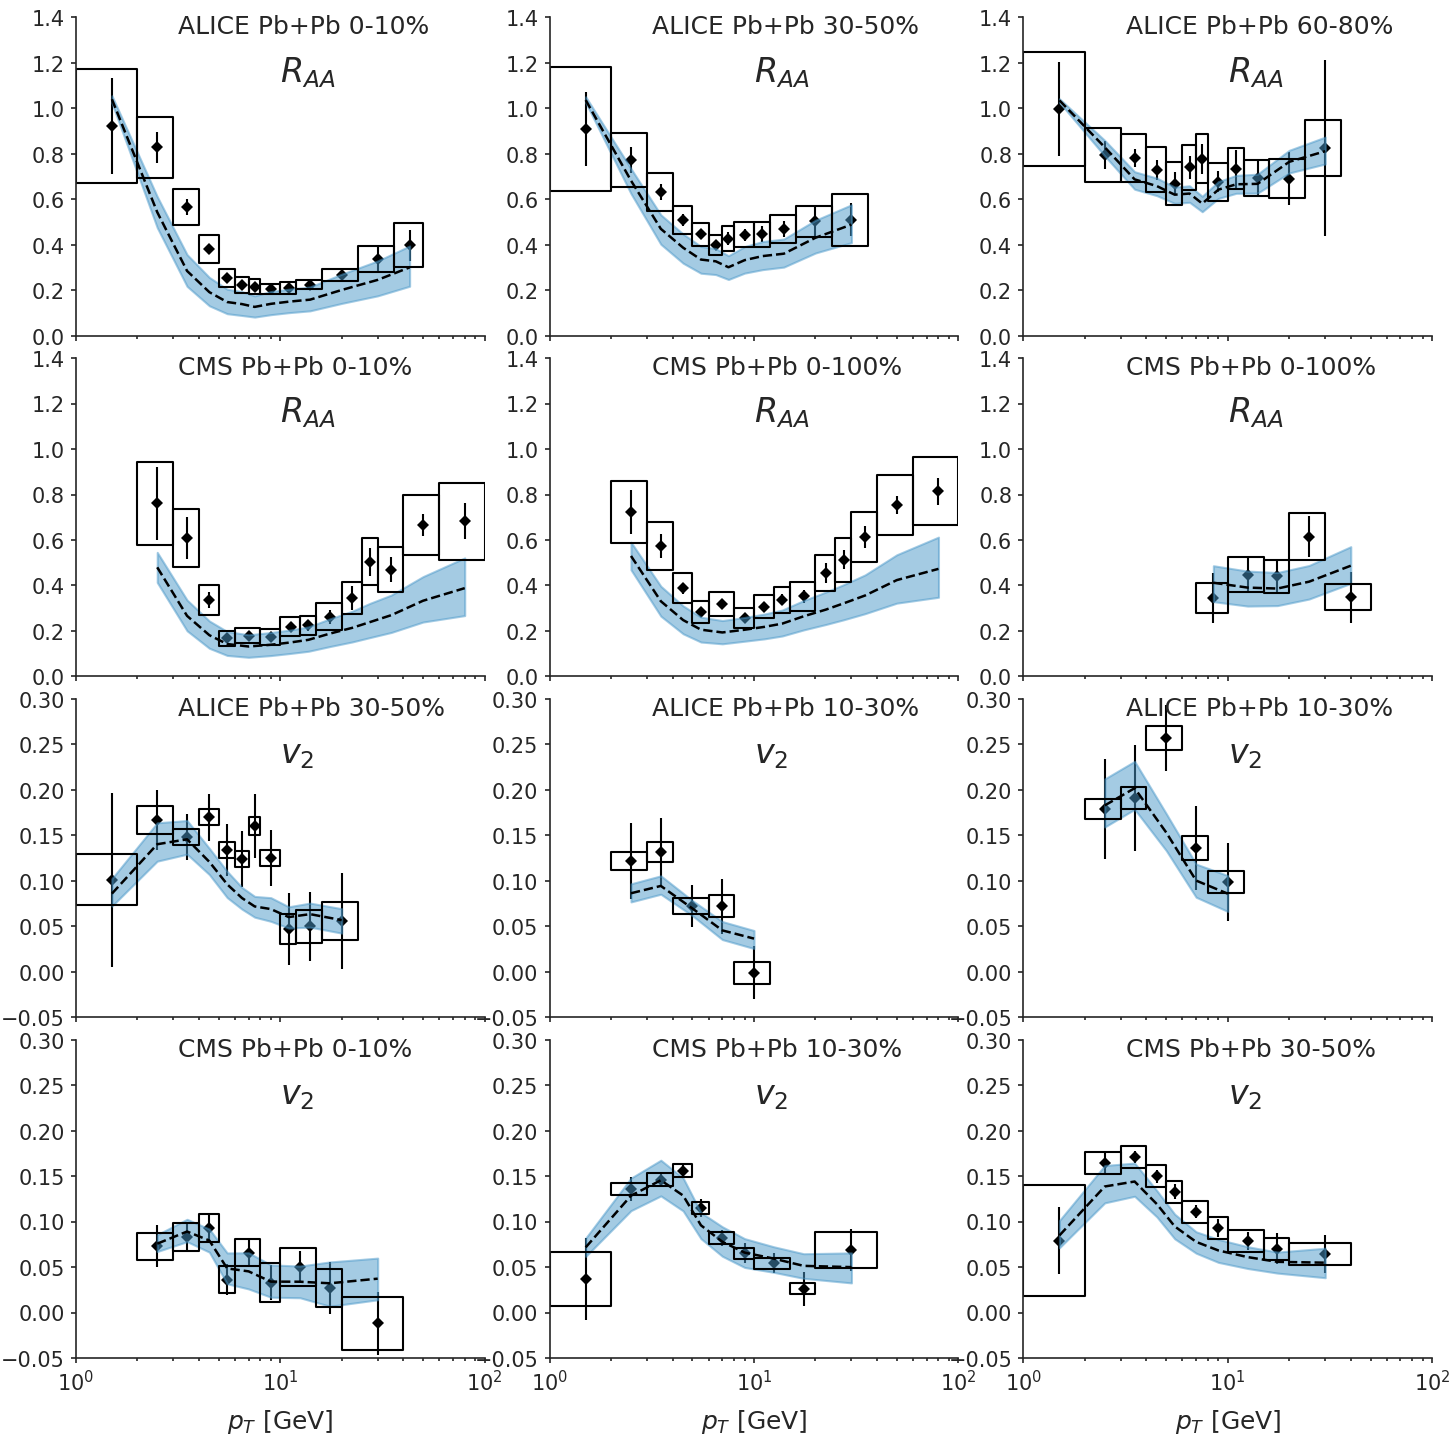
\includegraphics[width=\textwidth]{obs_posterior_LHC.png}
\caption{•}
\label{fig:new:obs_posterior_LHC}
\end{figure}

\paragraph{Posterior observables} The global level of agreement between the calibrated model and the data are shown in figure \ref{fig:new:obs_posterior_LHC} for LHC energy, and figure \ref{fig:new:obs_posterior_RHIC} for RHIC energy.
The both the $D$-meson and the $B$-meson $R_{AA}$ at the LHC energy is well described by the calibrated model, while $v_2$ is systematically below the data.
At the RHIC energy, the $v_2$ has a better agreement; the magnitude of $R_{CP}$ (note that we only calibrated on the three data points above $p_T=5$ GeV) is correct, though the shape is too flat compared to the data.

\begin{figure}
\centering
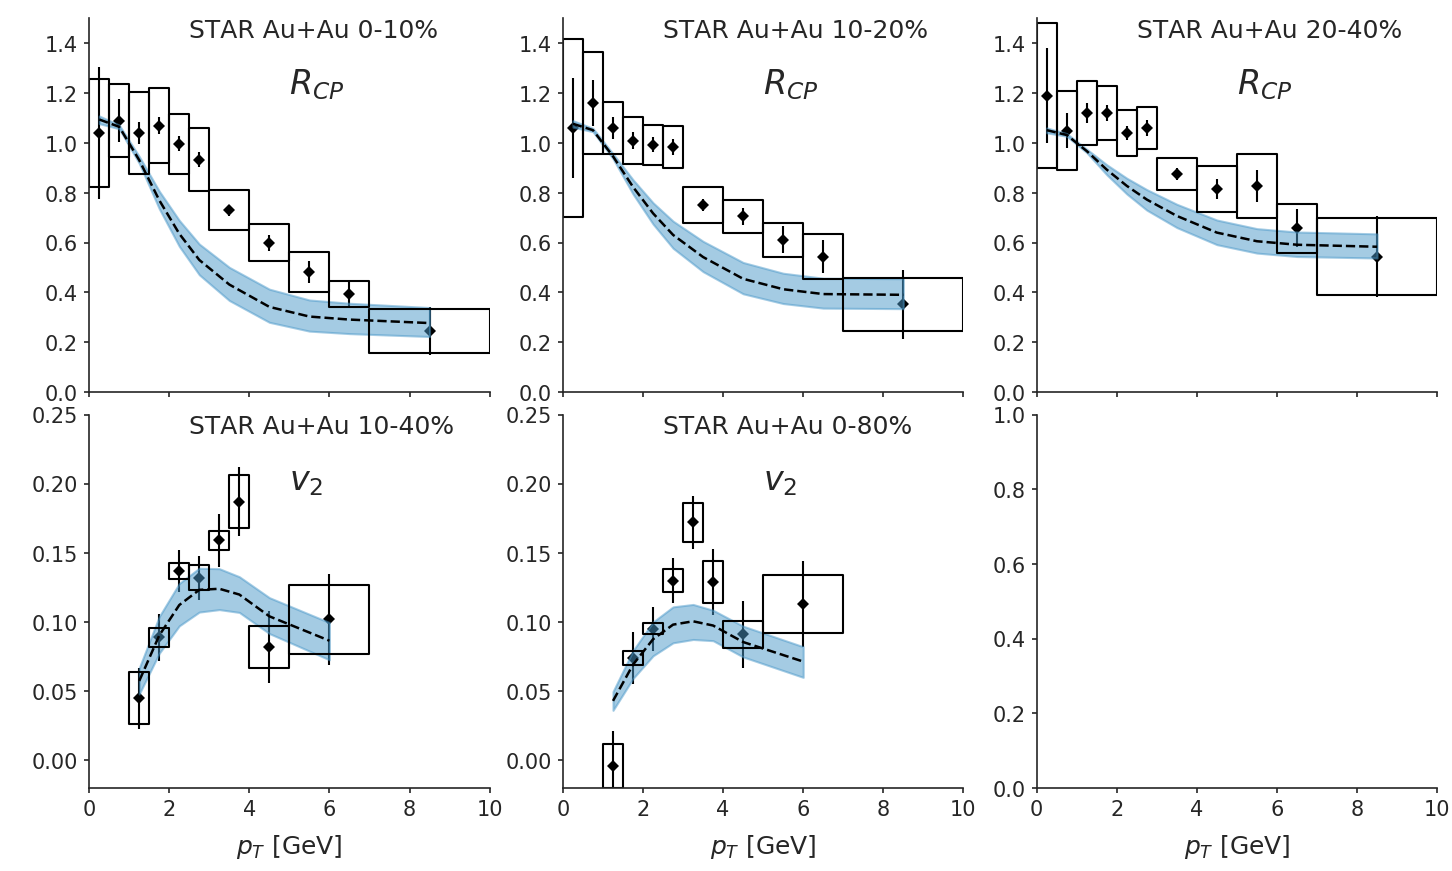
\includegraphics[width=\textwidth]{obs_posterior_RHIC.png}
\caption{•}
\label{fig:new:obs_posterior_RHIC}
\end{figure}

\begin{figure*}
\centering
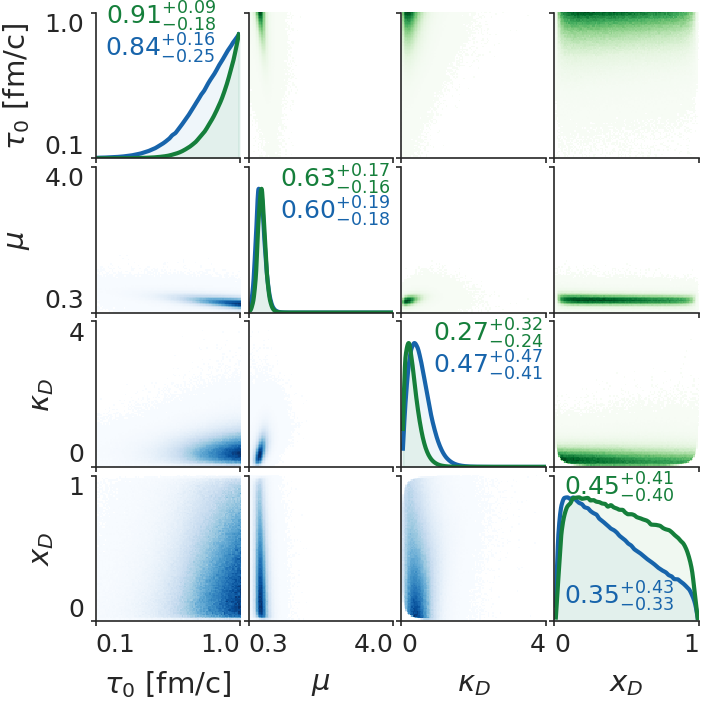
\includegraphics[width=\textwidth]{posterior.png}
\caption{•}
\label{fig:new:posterior}
\end{figure*}

\paragraph{Posterior distribution of parameters} Figure \ref{fig:new:posterior} shows the posterior distribution of the parameters.
The $\ln\mu$ parameter has a evident peak around $.99$, which correspond to $\mu \approx 2.7$.
Note that the means the preferred in-medium coupling is smaller than the extracted one from the previous analysis.
This is because the improved implementation of the radiave process produces more energy loss than the old one when the coupling is large, so a smaller value of $\alpha_s$ is needed to explain the data.
The resulting posterior of $\alpha_s$ (figure \ref{fig:new:posterior-alphas}) suggests an effective in-medium coupling from 0.20 to 0.33 at $T=300$ MeV.
Though the preferred $\alpha_s \sim 0.3$ is smaller than the previous one, $g\sim 2$ is still large, but this extracted coupling constant is much closer to phenomenological values used by other studies [].
The energy loss starting is preferred to be about half of the hydrodynamic starting time.
The switching scale parameter do not have a strong preference as long as it is not too large, which is consistent with our model construction that physical processes should be weakly depends on this switching scale between diffusion and scattering modeling.
The matching parameter $R_v$ is not very well constrained, as we have shown it only affects very high-$p_T$ observables.

\begin{figure}
\centering
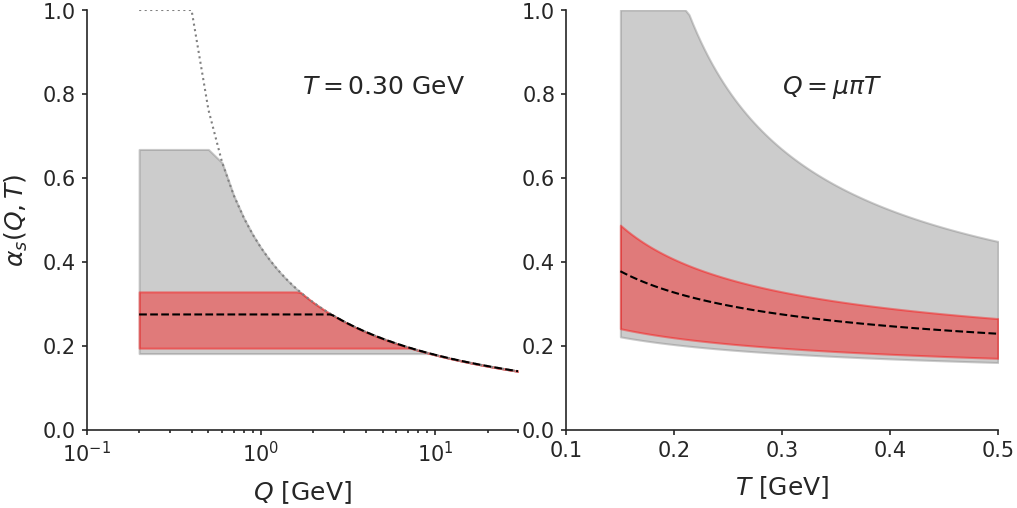
\includegraphics[width=.7\textwidth]{alpha_s_posterior.png}
\caption{•}
\label{fig:new:posterior-alphas}
\end{figure}

We plotted the 90\% credible range of the posterior transport parameters $\hat{q}, \hat{q}_L$ as the red bands in figure \ref{fig:new:posterior-qhat}.
The figure is arranged similarly to its prior plot.
The transport parameters is nicely constrained compare to its prior range (gray bands), and is comparable to the earlier extraction by the JET Collaboration \footnote{Note that the JET Collaboration extracts the light quark $\hat{q}$. However, at $p_T = 10$ GeV, the mass effect of the charm is small and these two numbers should be comparable.}.
We also present a first extraction of the longitudinal transport parameter. 
And it is quite anisotropic, similar to the pure weakly coupled expectation.

For the heavy quark spatial diffusion constant, since it is related to $\hat{q}$ in the zero momentum limit. 
Such an extraction is essentially an extrapolation of our parametrization, and can be sensitive to the detailed choice of the ansatz. 
Nevertheless, the extraction is compared to varies lattice calculations [] in  figure \ref{fig:new:posterior-Ds}.
Our extraction (red band for 90\% credible region) agrees with the lattice calculation in the static limit of the heavy quark; while calculation using dynamical charm quark gives a much lower value.


\begin{figure}
\centering
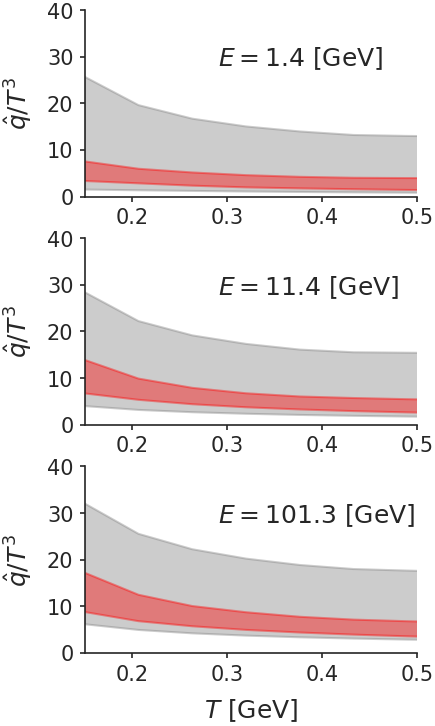
\includegraphics[width=.5\textwidth]{qhat_posterior.png}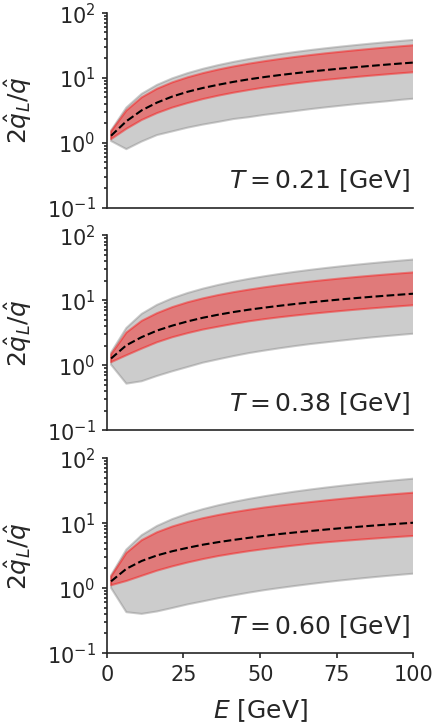
\includegraphics[width=.5\textwidth]{ER_posterior.png}
\caption{•}
\label{fig:new:posterior-qhat}
\end{figure}


\begin{figure}
\centering
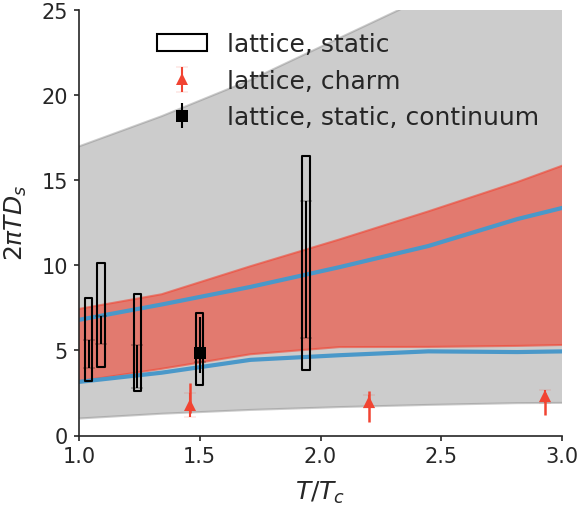
\includegraphics[width=.7\textwidth]{Ds_posterior.png}
\caption{•}
\label{fig:new:posterior-Ds}
\end{figure}

\paragraph{Prediction with high-likelihood parameter set}

